% Chapter 4

\chapter{Experimental Setup} % Write in your own chapter title
\label{Chapter4}
\lhead{Chapter 4. \emph{Experimental Setup}} % Write in your own chapter title to set the page header

Since the Mission Planning problem is so complex and recent in the state of the art, there does not exist datasets or benchmarks available. For this reason, some simple datasets have been developed.

In the following sections, we explain the implemented datasets for missions (including the topology of the mission scenario) and teams of \glspl{uav}, and the different schemas considered according to the temporal preferences between tasks.

\section{Missions datasets}
There has been designed 10 missions, each one composed by an increasing number of tasks from 1 to 10, i.e the first mission has one task; the second, two tasks; and so on. Table \ref{table:missions} shows the 10 considered tasks, where the first mission will execute task with ID T1; the second will execute tasks with IDs T1 and T2; and so on. This table shows the duration of the tasks instead of the start and end times. These times will be fixed on the experimental phase depending on the number of dependencies between the tasks. The action IDs come from Table \ref{table:taskActions}.

\begin{table}[h]
\caption{\gls{uas} mission with 10 tasks}
\label{table:missions}
\centering
\begin{tabular}{|c|c|c|c|c|c|}
\hline
Task ID & Action ID & Duration(min) & \begin{minipage}{1in}
    \vskip 4pt
    \centering
    Zone altitude\\
    window (km)
    \vskip 4pt
\end{minipage} & \begin{minipage}{1in}
    \vskip 4pt
    \centering
    Mean speed\\
    (km/h)
    \vskip 4pt
\end{minipage} & \begin{minipage}{1in}
    \vskip 4pt
    \centering
    Restricted\\
    zone?
    \vskip 4pt
\end{minipage}\\
\noalign{\hrule height 2pt}
T1 & A0 & 25 & {$[1.5-5]$} & 100 & NO \\
\hline
T2 & A2 &  20 & {$[1.5-5]$} & 100 & NO \\
\hline
T3 & A1 & 30 & {$[2.5-6.15]$} & 100 & YES \\
\hline
T4 & A0 & 25 & {$[0.5-3.75]$} & 100 & NO \\
\hline
T5 & A2 & 35 & {$[0.5-3.75]$} & 100 & NO \\
\hline
T6 & A1 & 30 & {$[3.85-5]$} & 100 & NO \\
\hline
T7 & A1 & 25 & {$[3.85-5]$} & 100 & NO \\
\hline
T8 & A1 &  12 & {$[1.5-5]$} & 100 & NO \\
\hline
T9 & A0 & 20 & {$[1.5-5]$} & 100 & NO \\
\hline
T10 & A2 & 25 & {$[2.5-6.15]$} & 100 & YES \\
\hline
\end{tabular}
\end{table}

In this approach, we consider the simple topology specified in Figure \ref{fig:topology}, where coloured areas represent the areas where tasks are performed and helicopters represent the airports where \glspl{uav} are situated at the beginning of the mission. In this scenario, there are four areas and four airports.

	\begin{figure}[!h]
		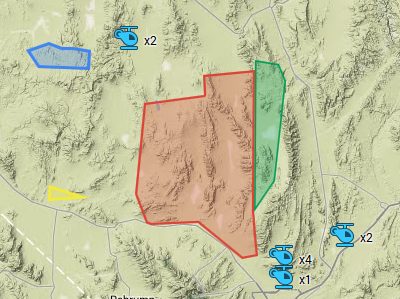
\includegraphics[width=0.8\textwidth]{./Figures/topology.png}
		\centering
		\caption{Topology of the scenario where missions are performed.}
		\label{fig:topology}
	\end{figure}


\section{\glspl{uav} datasets}
Different scenarios for solving the missions have been prepared with an increasing number of \glspl{uav} able to perform the tasks. The tasks contain several constraints, so when the number of tasks is very high, a high number of \glspl{uav} is also needed, mainly because of the fuel constraints. There has been considered groups of 1 to 9 vehicles available to perform the tasks (see Table \ref{table:uavs}). For a scenario with 1 vehicle, we use \gls{uav} with ID U1; for a scenario with 2 vehicles, \glspl{uav} with IDs U1 and U2; and so on.

\begin{table}[h]
\caption{Team of 9 available \glspl{uav}}
\label{table:uavs}
\centering
\begin{scriptsize}
\begin{tabular}{|c|c|c|c|c|c|c|}
\hline
\begin{minipage}{0.2in}
    \vskip 4pt
    \centering
    \gls{uav}\\
    ID
    \vskip 4pt
\end{minipage} & \begin{minipage}{0.7in}
    \vskip 4pt
    \centering
    Cruise speed\\
    window (km/h)
    \vskip 4pt
\end{minipage} & \begin{minipage}{0.6in}
    \vskip 4pt
    \centering
    Altitude\\
    window (km)
    \vskip 4pt
\end{minipage} & \begin{minipage}{0.7in}
    \vskip 4pt
    \centering
    Restricted zone\\
    permission
    \vskip 4pt
\end{minipage} & \begin{minipage}{0.5in}
    \vskip 4pt
    \centering
    Fuel consume\\
    (L/km)
    \vskip 4pt
\end{minipage} & \begin{minipage}{0.4in}
    \vskip 4pt
    \centering
    Initial\\
    Fuel (L)
    \vskip 4pt
\end{minipage} & Sensors Available \\
\noalign{\hrule height 2pt}
U1 & {$[90-110]$} & {$[0.3-6.5]$} & YES & 0.159 & 97.52 & \begin{minipage}{2in}
    \vskip 4pt
    \begin{itemize}
    	\item Camera EO/IR
    	\item Radar SAR
    	\item Communications Equipment
    \end{itemize}
    \vskip 4pt
\end{minipage} \\
\hline
U2 & {$[90-110]$} & {$[0.3-6]$} & NO & 0.159 & 58.48 & \begin{minipage}{2in}
    \vskip 4pt
    \begin{itemize}
    	\item Camera EO/IR
    \end{itemize}
    \vskip 4pt
\end{minipage} \\
\hline
U3 & {$[110-190]$} & {$[0.8-10]$} & YES & 0.2 & 140.23 & \begin{minipage}{2in}
    \vskip 4pt
    \begin{itemize}
    	\item Camera EO/IR
    	\item Radar SAR
    \end{itemize}
    \vskip 4pt
\end{minipage} \\
\hline
U4 & {$[90-110]$} & {$[0.3-6]$} & YES & 0.159 & 47.12 & \begin{minipage}{2in}
    \vskip 4pt
    \begin{itemize}
    	\item Camera EO/IR
    \end{itemize}
    \vskip 4pt
\end{minipage} \\
\hline
U5 & {$[90-110]$} & {$[0.3-6]$} & NO & 0.159 & 101.48 & \begin{minipage}{2in}
    \vskip 4pt
    \begin{itemize}
    	\item Camera EO/IR
    	\item Radar SAR
    	\item Communications Equipment
    \end{itemize}
    \vskip 4pt
\end{minipage} \\
\hline
U6 & {$[90-110]$} & {$[0.3-6]$} & NO & 0.159 & 101.37 & \begin{minipage}{2in}
    \vskip 4pt
    \begin{itemize}
    	\item Camera EO/IR
    	\item Radar SAR
    	\item Communications Equipment
    \end{itemize}
    \vskip 4pt
\end{minipage} \\
\hline
U7 & {$[90-110]$} & {$[0.3-6]$} & NO & 0.159 & 58.15 & \begin{minipage}{2in}
    \vskip 4pt
    \begin{itemize}
    	\item Camera EO/IR
    \end{itemize}
    \vskip 4pt
\end{minipage} \\
\hline
U8 & {$[110-190]$} & {$[0.8-10]$} & YES & 0.2 & 140.23 & \begin{minipage}{2in}
    \vskip 4pt
    \begin{itemize}
    	\item Camera EO/IR
    	\item Radar SAR
    \end{itemize}
    \vskip 4pt
\end{minipage} \\
\hline
U9 & {$[90-110]$} & {$[0.3-6]$} & YES & 0.159 & 47.12 & \begin{minipage}{2in}
    \vskip 4pt
    \begin{itemize}
    	\item Camera EO/IR
    \end{itemize}
    \vskip 4pt
\end{minipage} \\
\hline
\end{tabular}
\end{scriptsize}
\end{table}


\section{Temporal schemas}\label{temporalschemas}
Three scenarios have been generated with different temporal schemas based on the time dependencies between the tasks. Figure \ref{fig:tempoNoDep} shows an scenario with no time dependencies between tasks, i.e. the tasks do not collide in time. Figure \ref{fig:tempo1Dep} shows an scenario where each task collides in time with the previous task, i.e. there are $n-1$ temporal dependencies, being $n$ the number of tasks. Finally, when each task collides in time with the two previous tasks, i.e. there are $2(n-1)-1$ temporal dependencies, we have the scenario shown in Figure \ref{fig:tempo2Dep}.

	\begin{figure}[!h]
	\centering
		\begin{subfigure}[b]{0.9\textwidth}
			\includegraphics[width=\textwidth]{./Figures/tempoNoDep.png}
			\centering
			\caption{No dependencies}
			\label{fig:tempoNoDep}
		\end{subfigure}
		\begin{subfigure}[b]{0.9\textwidth}
			\includegraphics[width=\textwidth]{./Figures/tempo1Dep.png}
			\centering
			\caption{Dependency of each task with the previous task.}
			\label{fig:tempo1Dep}
		\end{subfigure}
		\begin{subfigure}[b]{0.9\textwidth}
			\includegraphics[width=\textwidth]{./Figures/tempo2Dep.png}
			\centering
			\caption{Dependency of each task with the two previous tasks.}
			\label{fig:tempo2Dep}
		\end{subfigure}
		\caption{Three schemas of the scenarios based on the number of temporal dependencies between the tasks.}
		\label{fig:tempo}
	\end{figure}
	
These schemas will be compared in the experimental phase (see Chapter \ref{Chapter5}) in order to observe the scalability of the problem as the number of temporal dependencies increase.